
\documentclass[sigconf,final]{acmart}

\AtBeginDocument{%
  \providecommand\BibTeX{{%
    \normalfont B\kern-0.5em{\scshape i\kern-0.25em b}\kern-0.8em\TeX}}}
%% Rights management information.  This information is sent to you
%% when you complete the rights form.  These commands have SAMPLE
%% values in them; it is your responsibility as an author to replace
%% the commands and values with those provided to you when you
%% complete the rights form.
\setcopyright{acmlicensed}
\copyrightyear{2024}
\acmYear{2}
\usepackage{tabularx}
\usepackage{multirow} % 合并行
\usepackage{booktabs}
\usepackage{amsmath}
\usepackage{booktabs}
\begin{document}
\fancyfoot[C]{\thepage} 
\fancyfoot[R]{%
    \ifnum\value{page}=3 
        \href{https://doi.org/10.7910/DVN/6BPCXN}{\textsuperscript{1}{https://doi.org/10.7910/DVN/6BPCXN}}%
    \fi
    \ifnum\value{page}=4 
        \href{https://github.com/2020213484/TCA_Keystroke}{\textsuperscript{2}{https://github.com/2020213484/TCA_Keystroke}}%
    \fi
}
\title{Cross-semester Student's Coding Performance Prediction by Keystroke Analysis with Transfer Component Analysis}

\author{Ziyang Ji}
\affiliation{%
  \institution{University of Auckland}
  \city{Auckland}
  \country{New Zealand}}
\email{zji009@aucklanduni.ac.nz}

\author{Yunhao Wang}
\affiliation{%
  \institution{University of Auckland}
  \city{Auckland}
  \country{New Zealand}}
\email{nway818@aucklanduni.ac.nz}

\author{Yuxiang Huang}
\affiliation{%
  \institution{University of Auckland}
  \city{Auckland}
  \country{New Zealand}}
\email{yhua963@aucklanduni.ac.nz}

\author{Yu Tang}
\affiliation{%
  \institution{University of Auckland}
  \city{Auckland}
  \country{New Zealand}}
\email{ytan173@aucklanduni.ac.nz}


\renewcommand{\shortauthors}{Ziyang Ji, Yunhao Wang, Yuxiang Huang and Yu Tang.}


\begin{abstract}
Programming has become an essential skill for STEM students nowadays, and many students find it hard to get started. Personal assistance is needed to help struggling students be better supported in their programming learning process. Student performance prediction is an important step for personal assistance. Several prior works have been trying to predict students' coding performance by analyzing their keystroke data in the coding process. However, almost all of these works only focus on the prediction task of the data of the same semester. It is obvious that this kind of work could hardly be applied to practical applications as students' scores are unavailable until the semester ends. To fill the gap between existing works and practical applications, we use the data from the same course but the previous semester to predict students' scores in the current semester. We apply the domain adaptation method like TCA in the machine learning area to boost the model's performance on cross-semester prediction tasks. Our results suggest that the domain adaptation method can help improve predicting students' coding performance when only previous semester data is available for training the model. However, our results suggest that even if the domain adaptation method is applied, it is still a big problem to predict students' coding performance in practical application situations.

\end{abstract}


\ccsdesc[500]{ Social and professional topics~computing education.}


%%
%% Keywords. The author(s) should pick words that accurately describe
%% the work being presented. Separate the keywords with commas.
\keywords{Keystroke Analysis, XGBoost, Domain Adaptation, Machine Learning}
\maketitle
\thispagestyle{fancy}
\section{INTRODUCTION}
With the rapid development of information technology, programming education has become an integral part of modern higher education systems. In today’s era, mastering programming skills 
have transcended the realm of computer science and become an essential core skill in many industries. Despite the increasing importance of programming education, it faces several challenges in practice. The primary issue is the high failure rate of programming courses, which has become a hot topic in the education sector [2, 10]. Research indicates that the dropout rate for introductory computer science courses (CS1) is significantly higher than that of other STEM courses, and this problem is widespread across different regions and educational systems globally [2]. Additionally, the significant differences in students’ programming abilities cannot be ignored, which may be influenced by various factors such as individual traits, learning motivation, cognitive tendencies, and educational resources [9, 15]. Educators need to explore how to efficiently cultivate students’ ability to analyze and solve problems, which is crucial for the success of programming education [12].

In this context, educators and researchers are facing an important challenge: How to accurately measure students’ performance in programming and provide targeted learning support based on 
these performances [2, 10]. With the rapid development of emerging research fields such as learning analytics and educational data mining, scholars now have the opportunity to utilize the vast amount of keystroke data generated by students during the learning process to conduct more educational effectiveness evaluations and customized learning support. By examining students’ keyboard inputs and mouse movements during coding tasks, educators can give an evaluation of students’ coding performance based on their keystroke data[2, 6, 10, 15]. 

However, most of these existing works mainly focused on predicting students’ final scores on only one semester’s dataset. These works usually try to build a training set, validation set, and testing set on only one semester’s dataset by splitting it into 3 different parts, with different sets having different students’ keystroke data. However, it is a significant problem that most of the existing research does not take the practical application situation into consideration. In a practical application situation, for the semester where we would like to apply keystroke data for prediction, no label information can be provided until the end of the whole semester. Due to such reasons, almost all the existing research works could hardly be used to predict students’ coding performance in a practical setting to help teachers discover the students in need. 

To fill the gap between existing research and practical application, we try to use the model trained from the dataset of the same course but the previous semester to predict students’ coding performance in the current semester. It is obvious that there exists a gap between previous semester data and current semester data; simply using the model trained from the previous semester’s data could hardly generalize well on the current semester’s data. To reduce such a gap, we apply domain adaptation methods from the machine learning area, which aims to improve the performance of a model on a target domain by leveraging knowledge from a related source domain in order to help improve the prediction performance of the model in the current semester. 

To evaluate the gap between existing research works and practical application and how well could domain adaptation methods be applied to enhance prediction performance, we train and evaluate models on a dataset from two continuous semesters of the same course. We investigate two research questions(RQs):

\textbf{RQ1.} How well could the models behave on current semester data if the models are trained directly from the same course but previous semester data?

\textbf{RQ2}. How well could the prediction performance in the current semester be improved by applying domain adaptation methods to the model from the previous semester?

In section 2, we describe related work, including existing works on applying keystroke data for coding performance prediction and domain adaptation methods from the machine learning area. Next, in section 3, we introduce our datasets and the context where they were collected. In section 4, we describe the methods we adopted. Then, in section 5, we show our results. In section 6 we talk about the limitations of our work. Finally, in section 8, we make a conclusion.

\section{RELATED WORK}
In this section, we will talk about the previous works on students’ coding performance prediction as well as some traditional works in the domain adaptation area.

\subsection{Students’ coding performance prediction}
\subsubsection{Keystroke features correlate with Programming Performance}

Pereira et al. [2] found effective programming practices like error handling and extended coding times linked to better learning outcomes, while copy-paste activities were detrimental for beginners. Munson et al. [3] associated more coding time and frequency with higher grades and noted a negative correlation between syntax errors and grades. Leinonen et al. [4] reported moderate to weak correlations between time-on-task metrics and exam scores. Khan et al. [6] observed higher assignment grades for students using specific keys more frequently, and Casey et al. [14] noted stable correlations between keystroke metrics and exam performance from week 6 onwards. Shrestha et al. [9] found more frequent pausing predicted lower exam scores. Pereira et al. [10] identified behaviors like fewer deletions and less copy-pasting as effective, while a high error quotient indicated problem-solving challenges. Leinonen et al. [15] suggested quick character type switching negatively impacted exam performance. Carter et al. [17] found PSM transition sequences correlated with course performance, and Edwards et al. [18] showed error recovery speed improved with advancing programming skills. Matsumoto et al. [19] discovered a positive correlation between numeric key usage and scores, but more time on testing, compiling, and web browsing was linked to lower programming performance.
\begin{figure*}[ht]
  \centering
  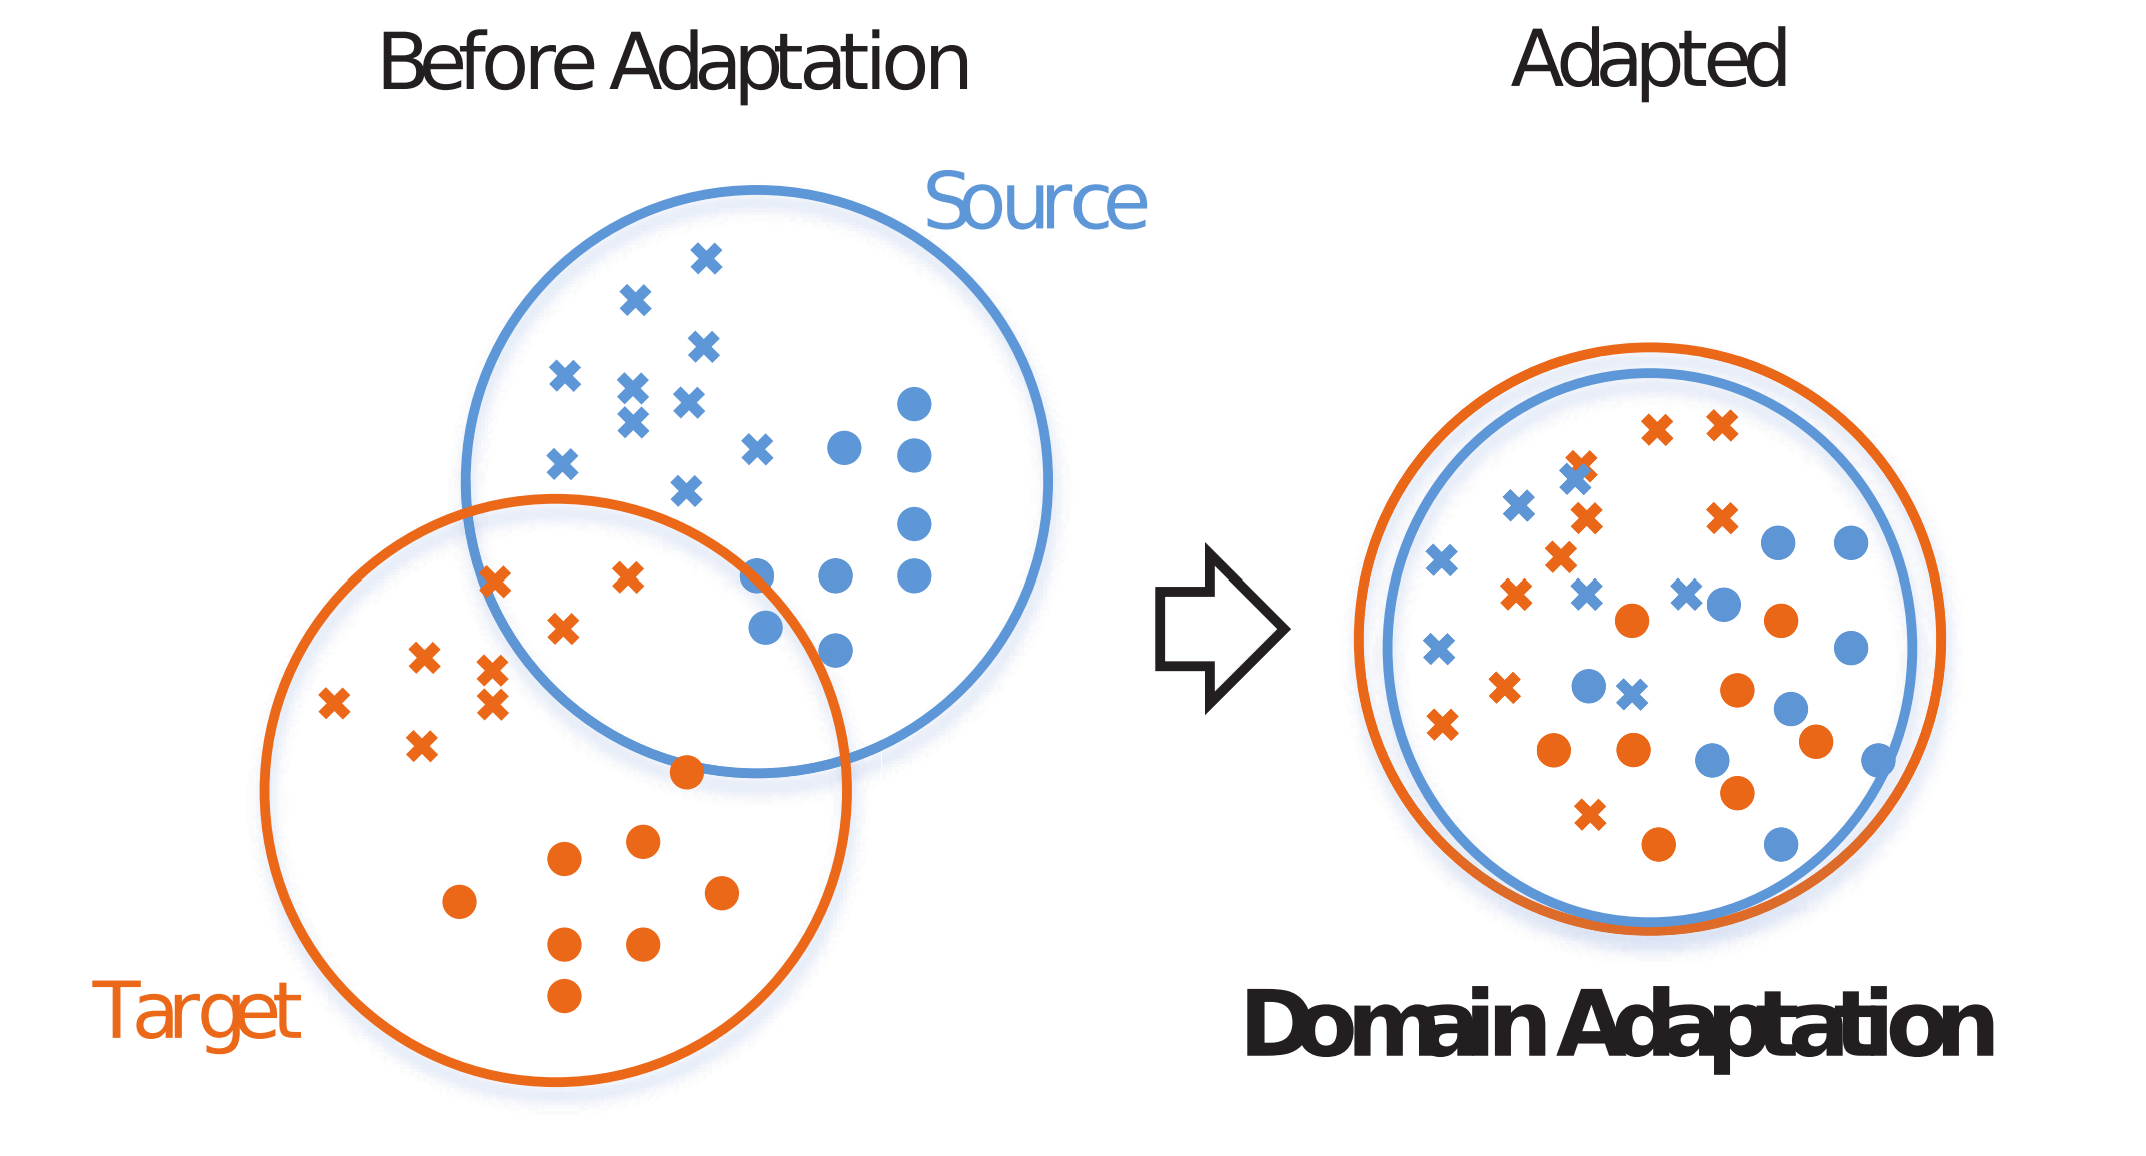
\includegraphics[width=\linewidth]{domain.png}
  \caption{Illustration of domain adaptation, from Zhu et al. [23]}
  \label{fig:imglabel}
\end{figure*}

\subsubsection{ Models for Coding performance prediction with Keystroke data:}


Watson et al. [1] used the Watwin algorithm, which explained 42.49\% of grade variance. Munson et al. [3] developed linear regression models, identifying key variables and using an algorithm to select the best models for accurate predictions. Leinonen et al. [4] compared random forest and logistic regression models, finding higher accuracy with fine-grained Time-on-Task (ToT). Khan et al. [6] combined Isolation Forest anomaly detection with Random Forest, achieving an 80\% accuracy rate. Pereira et al. [10] cleaned data and used XGBoost, obtaining an 81.3\% accuracy and ROC-AUC of 0.89 in predicting introductory course outcomes. Casey et al. [14] compared models with and without keystroke data, with the extended model showing better performance. Pullar-Strecker et al. [16] evaluated multiple machine learning models across different datasets, noting high variance in model performance and the hard to generalize problem.


\subsection{Domain adaptation}
Domain adaptation is a machine learning technique used to address a common challenge known as the domain shift problem[20]. This problem arises when a model trained on data from one source domain performs poorly on data from a different target domain.


There are various approaches to domain adaptation, including feature-based methods, where the model learns to extract features that are invariant across domains, and instance-based methods, where the model reweights or selects instances from the source domain to better match the target domain [20]. Additionally, adversarial learning techniques have gained popularity in domain adaptation, where a domain discriminator is trained to distinguish between source and target domain data while the model is simultaneously trained to confuse the discriminator [20].


We mainly adopt feature-based methods in our work, such as component analysis (TCA)[21]. TCA (Transfer Component Analysis) is a domain adaptation technique that learns a feature transformation to align the source and target domain distributions in a lower-dimensional subspace, reducing the Maximum Mean Discrepancy (MMD) between them and enabling effective knowledge transfer. It is built on the assumption that the source domain and target domain share the same conditional distribution P(Y|X) and different marginal distribution P(x), i.e$$P_{\text{source}}(Y|X) = P_{\text{target}}(Y|X)$$ and $$P_{\text{source}}(X)\neq  P_{\text{target}}(X)$$, where Y is the label variable and X is the input feature variable. In this situation $$P_{\text{source}}(X,Y)\neq P_{\text{target}}(X,Y)$$ since $$P(X,Y)=P(Y|X)\cdot P(X)$$. As the joint distribution P(Y, X) is different in the source domain and target domain, it can be hard to train a model from a training set that generalizes well on the target source. However, through Transfer Component Analysis, the original features from source domain and target domain are projected into a subspace where the projected feature marginal distribution $$P_{\text{source-projected}}(X)\approx P_{\text{target-projected}}(X)$$, thus we have $$P_{\text{source-projected}}(X,Y)\approx P_{\text{target-projected}}(X,Y)$$. So the model trained on the TCA-based projected features can have a better generalization ability compared with the model trained in the original feature space.
\begin{table*}[h]
\centering
\caption{The features used in our analysis.}
\begin{tabular}{r|l} % r代表右对齐,l代表左对齐
\toprule
Name & Description\\ \hline
First k-th moments based on the frequency of the 1-gram keystrokes & 
\\
First k-th moments based on the frequency of the 2-gram keystrokes & 
\\
Average delay time for keystrokes & Average delay time for keystrokes except for some outlier keystroke \\
Fine-grained time spent on assignment & Actual time spent completing assignments \\
Coarse-grained time spent on assignments & Total time spent completing assignments \\
Total count of keystrokes & Number of all the keystroke events recorded \\
Actual total length of the program code & Number of all the characters in each assignment \\
Percentage of 'delete' key usage & Percentage of using 'delete' key among all the keystroke events \\
Scores for each assignment&  \\
Number of micro pauses & Number of keystroke events with time interval length 2-15 seconds\\
Number of short pauses & Number of keystroke events with time interval length 15-180 seconds \\
Number of mid pauses & Number of keystroke events with time interval length 3-10 minutes \\

\bottomrule
\end{tabular}
\end{table*}

\section{CONTEXT}
In this study, we evaluate students’ coding performance prediction methods on two datasets from the same course, which are from two continuous semesters.
The dataset originates from the CS1 (CS 1400) course offered in the spring and fall of 2019 at Utah State University. The data was collected by Professors John Edwards and Chad Mano from the Department of Computer Science at Utah State University from students who participated in the course and research [5, 13]. The dataset is available online \textsuperscript{1}.

The CS 1400 course is an introductory computer science course that teaches basic problem-solving, coding, and program development, as well as some foundational algorithm analysis and data structures. In this course, students use Python as the programming language for development and learning. The research and data collection mainly focused on the first five weeks of the fall semester. The data was collected through a customized Python IDE with data collection capabilities, Phanon, as students worked on course exams and assignments. 

During the 5-week course period, students were assigned to complete one assignment per week. Each assignment included two tasks, with each task containing a small programming task accompanied by a detailed grading rubric. Additionally, each assignment provided instructional examples similar to the task content (with answers) for reference. The programming tasks in the assignments mostly involved Turtle graphics, simple user interactions through step-by-step user inputs, solving mathematical problems, and other routine entry-level programming tasks, covering knowledge such as Turtle graphics, variables and operators, data types and type conversion, string processing, function writing, basic software development processes, basic selection and conditional judgments, and basic loop writing.

In addition to recording students' keystroke data while completing programming tasks in the course, students participating in the research were also asked to fill out surveys at the beginning and end of the course and occasionally during the course to complement the research. The keystroke data from filling out the surveys were also recorded and differentiated from the data generated from programming exercises with different tags ("English" for surveys and "Python" for programming exercises) [5].

The study has been reviewed and approved by the Institutional Review Board (IRB) for the protection of human research participants at Utah State University. In the research, the collected data will be anonymized and de-identified. Moreover, students can voluntarily withdraw from the research or the course in which the research is conducted, and the corresponding recorded data will be excluded [7].

The dataset is mainly composed of two parts. The first part is about student’s keystroke data in their assignments. The useful information in keystroke data includes EventID, SubjectID, AssignmentID, EventType, X-Keystroke, InsertText, DeleteText, SourceLocation, ClientTimestamp, EditType and X-semester. EventID is the ID of all students’ keystroke ID. SubjectID is the ID of students taking this course. AssignmentID is the ID of the assignment. EventType is the ID of the event recorded in the Phanon. X-Keystroke is the keystroke that students press on the keyboard. InsertText is the text students inserted at each step. DeleteText is the text students delete at each step. SourceLocation is the location of the keystroke at each step. ClientTimestamp records the time stamp of each keystroke event. EditType is the type of edition of each keystroke event. X-semester records the semester where the event happened. There are a total of 5130297 keystroke events in all, with 2329278 keystroke events in the spring semester and 2801019 keystroke events in the fall semester. 
\begin{table*}[h]
\centering
\caption{Metrics for different sets.}
\begin{tabular}{|c|c|c|c|c|} % r代表右对齐,l代表左对齐
\toprule
Metrics & Training Set &Validation Set &Testing Set Without TCA & Testing Set With TCA\\ \hline
 Accuarcy& 0.886 &0.633 &0.586 & 0.591\\ \hline
 Precision & 0.913 &0.685 &0.528 & 0.532\\ \hline
  Recall & 0.843 &0.517 &0.923 & 0.923\\ \hline
  F1  & 0.876 &0.567 &0.672& 0.675\\ 
\bottomrule
\end{tabular}
\end{table*}
\begin{figure*}[ht]
  \centering
  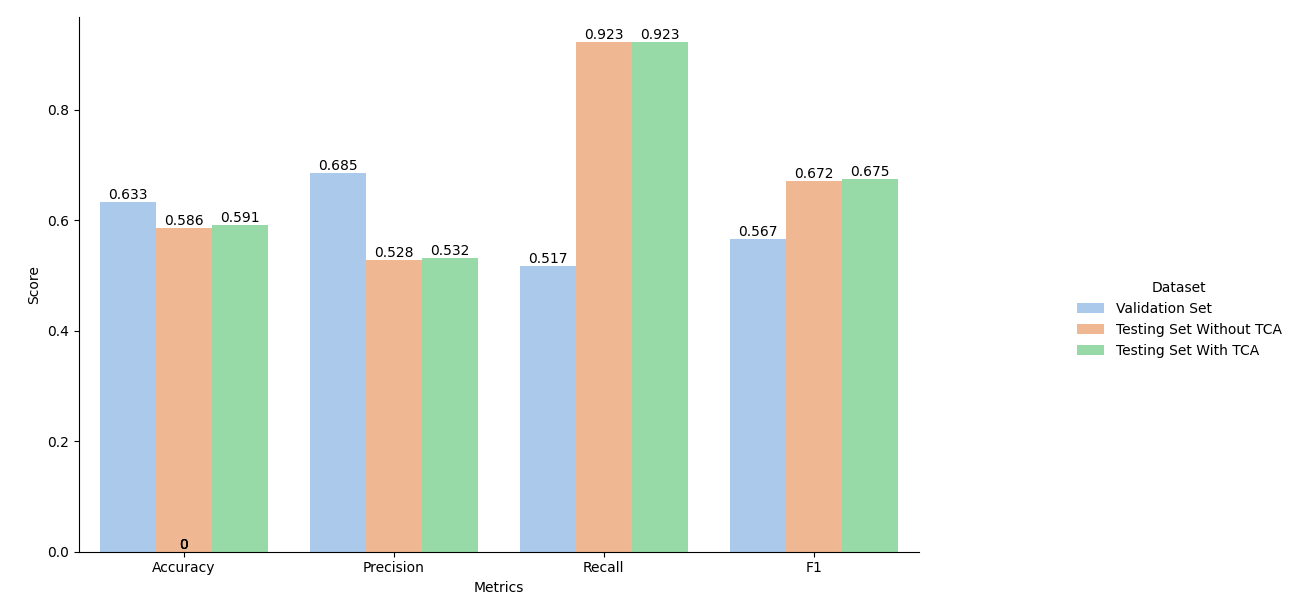
\includegraphics[width=\linewidth]{table3.png}
  \caption{The bar chart illustrates that the TCA-based domain adaptation method can improve the model performance slightly on the testing set. It also indicates the domain gap between data from different semesters.}
  \label{fig:imglabel}
\end{figure*}


The second part is about students’ scores on each assignment and exam. There are 5 assignments and 2 exams in total. Each of these assignments and exams has 100 marks. What is more, all the assignments and exams are recorded, whether they were completed by students in the spring semester or fall semester.

Due to the fact that there is no detailed information available online regarding the weightings for each assignment's grades and exam scores, it is impossible to calculate the final grades for each student. So we take the average score of two exams as the objective we need to predict in our research.



\section{METHODOLOGY}

We talk about our methodology in detail in this section. All of the analysis is performed in Python and will be available on Github\textsuperscript{2}. 


The dataset contains many incomplete information which may be harmful for further analysis. According to the second part of the dataset which records students’ scores in assignments and exams, we notice that many of the students failed to continue to the end of the semester. Moreover, some of the students only took one exam of a total of two exams. Thus, we cannot evaluate their coding performance fairly compared with those who took all the exams. Additionally, some of the students took the course both in the spring semester and fall semester, which may be because of their failure in the previous semester. All of the anomalous data we mentioned
above were deleted in our analysis to avoid interference from noise.

Then we extract features from the keystroke events collected by Python IDE Phanon. The features we extracted can be classified into two parts. The first part is keystroke information irrelevant features, and the second part is keystroke information relevant features. For the keystroke information irrelevant features, we take all the keystroke events into consideration, including the events where X-Keystroke value is NaN or blank. And for those keystroke information relevant features, we do not take the events where X-Keystroke value is NaN or blank into account.


We build 10 keystroke information irrelevant features in total:


1) The average delay time for keystrokes: The average delay time for keystrokes except for some outlier keystrokes. Similar to the previous work[16], we do not consider the keystroke events with time interval length in the top 0.3\%. It means that we only take the shortest 99.7\% delay time into account for average delay time computation according to the 3-sigma rule.


2) Fine-grained time spent on assignment: The actual time spent completing assignments, excluding time when assignments might not be worked on. Similar to the previous work[16], we do not consider the keystroke events with time interval length in the top 0.3\%. It means that we only take the shortest 99.7\% delay time into consideration, as long time intervals may indicate that students might not work on their assignments at that time.


3) Coarse-grained time spent on assignments: The total time spent completing each assignment, which is from the first keystroke to the last keystroke of each assignment.


4) The total count of keystrokes: The number of all the keystroke events recorded for each assignment. 


5) The actual total length of the program code: The number of all the characters in each assignment. 


6) The percentage of 'delete' key usage: The percentage of using the 'delete' key among all the keystroke events for each assignment. 


7) Scores for each assignment.


8) Number of micro pauses: Number of keystroke events with a time interval length of 2-15 seconds, which may indicate the student is thinking about the code on a low level or “locally” (e.g. syntax) [9].


9) Number of short pauses: Number of keystroke events with a time interval length of 15 seconds to 180 seconds, which may indicate that the student is involved in a higher-level process such as planning or revision [9].


10) Number of mid pauses: Number of keystroke events with a time interval length of 3-10 minutes, which may indicate that the student is disengaged or that they are going to an outside resource for help (e.g. YouTube, Stack Overflow, or course materials) [9].


\begin{figure*}[ht]
  \centering
  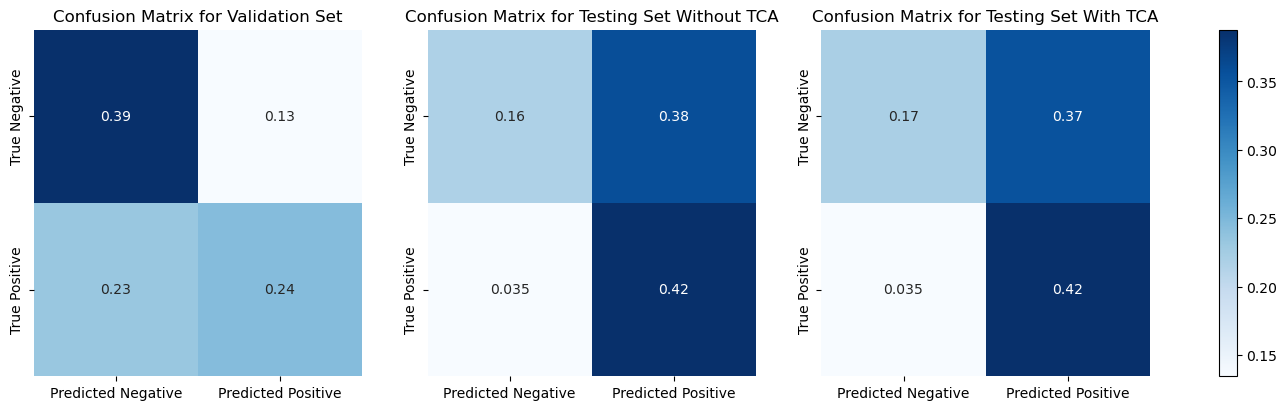
\includegraphics[width=\linewidth]{table4.png}
  \caption{Confusion matrices for validation set, testing set without TCA and testing set with TCA. The positive represents students below the average score and vice versa, as we only focus on the students with poor coding performance.}
  \label{fig:imglabel}
\end{figure*}

Furthermore, we build two major types of keystroke information-relevant features. We build features based on 1-gram and 2-gram keystroke frequency. Different from the previous works, we do not directly take frequency as the feature, which may potentially lead to the overfitting problem due to the great number of features. Instead, we consider the global statistical information about keystroke frequency. It is well-known that moment is a crucial statistical characteristic of a probability distribution, where each order of moment reflects various properties of the distribution. For example, the first moment E[X] represents mean; the second moment $E[X^2]$ represents variance; the third moment $E[X^3]$ represents skewness, indicating the asymmetry of the distribution; the fourth moment $E[X^4]$ represents kurtosis, describing the tailedness or peakedness of the distribution. We compute the first k-th moments $\left\{ E[X^i] \right\}_{i=1}^k$  of the probability distributions formed by the frequencies of occurrence of 1-gram and 2-gram keystrokes. K is chosen as 7 in our research.


1) First k-th moments based on frequency of the 1-gram keystrokes: We compute all the frequencies of 1-gram keystrokes for each assignment and for each student, which forms a probability distribution. Then we calculate the first k-th moments $\left\{ E[X^i] \right\}_{i=1}^k$ for each distribution, which reflects 1-gram keystroke’s global statistical information for each student on each assignment.


2) First k-th moments based on the frequency of the 2-gram keystrokes: To reduce the total computation, we first select the 50 most frequently occurring characters. Then we compute the occurrence time of 2-gram keystrokes formed by those 50 characters. Next, we select the 100 most frequently occurring 2-gram keystrokes for further analysis. In the end, we compute the k-th moments on the 2-gram keystrokes in the way same as the 1-gram keystrokes.


To sum up, we build 10 keystroke information irrelevant features and 2*k keystroke information relevant features. All of these features are established based on each assignment for each student. We only considered the first three assignments to build the features, for the reason that if we take all the assignments into account, time for helping students in need will be limited.

We then apply XGBoost[22] with quantile regression loss as the model for the prediction task. XGBoost is one of the best models for tabular data prediction tasks. We equip XGBoost with quantile regression loss  to enhance its performance, since quantile regression loss can provide prediction confidence intervals for the model, and enhance the model's robustness in the face of noise. 

We train the model with 2019 Spring semester data as the training set and validation set. We first train the model with a 5-fold cross-validation setting to find a good hyper-parameter for the model. Then, we apply the tuned hyper-parameter on the model and retrain the model on the merged dataset composed of the initial training set and validation set. 

To seek the answer to RQ1, we first test our model directly in the 2019 fall semester to figure out whether the model trained in the previous semester can generalize well in the current semester. To seek the answer to RQ2, we apply Transfer Component Analysis (TCA) to our input features. In our research, the 2019 Spring dataset is the source dataset, and the 2019 Fall dataset is the target dataset. We apply TCA to both features in the source dataset and target dataset, projecting original features from those datasets into a subspace, where the projected features from the source domain and target domain are aligned in the subspace. Then, we train our model on the projected features to figure out how well could the prediction performance in the current semester be improved by applying domain adaptation methods.




\section{RESULTS}
We mainly use four different metrics to evaluate our model’s performance, including accuracy, precision, recall and F1 value. Accuracy indicates the proportion of all samples that the model makes the correct prediction, precision indicates the proportion of true positive samples among the samples predicted as positive, and recall indicates the proportion of samples recognized as positive among all the positive samples. As we are only interested in those students who need help, we set the students whose scores in exams are below the average score as the positive samples and the students whose scores in exams are above the average score as the negative samples.

Our RQ1 aims to discover how well the model could behave on current semester data if models are only trained directly from the previous semester data. In order to solve this problem, we take the 2019 Spring data as the previous semester data and the 2019 Fall data as the current semester data. After the data cleaning process, there are 249 students’ information available in the spring semester and 198 students’ information available in the fall semester. We train the XGBoost model with quantile regression loss in the spring semester with 5-fold cross-validation, with the SelectKBest function from the sci-kit-learn package to choose the most important K features. Through cross-validation, we determined the best parameter K=54 in the SelectKBest function. 

The 5-fold cross-validation yields the following average metrics on the training set: an accuracy score of 0.886, a precision of 0.913, a recall of 0.843, and an F1 score of 0.876; and the following average metrics on the validation set: an accuracy score of 0.633, a precision of 0.685, a recall of 0.517, and an F1 score of 0.567. Then, we merge the training set and validation set into a new training set and retrain the model on the new training set with the same hyperparameters determined in the cross-validation stage. We directly test our model on the 2019 fall data and get the following average metrics on the testing set: an accuracy score of 0.586, a precision of 0.528, a recall of 0.923, and an F1 score of 0.672. 

Our RQ2 aims to discover how well could the model behaviour be improved by applying domain adaptation methods in cross-semester prediction tasks. We apply Transfer Component Analysis (TCA) as the domain adaptation method to better transfer the knowledge from the source domain to the target domain. In our research, the spring semester’s data forms the source domain, and the fall semester’s data forms the target domain. We use TCA to project the initial input features into a subspace, where the MMD distance of projected features from the source domain and target domain is minimized. We adopt the initial feature number K=54, which is determined in 5-fold cross-validation, as mentioned before. Then we train the model on the projected features of the spring semester data with projected feature number 20. We further test our model on fall semester data, with projected features as inputs. The average metrics on the testing set are as follows: an accuracy score of 0.591, a precision of 0.532, a recall of 0.923, and an F1 score of 0.675. The average metrics on the testing set with the TCA method adopted are obviously better than those without the TCA method.

\section{DISCUSSION}
Our first RQ sought to discover how well the model could behave on current semester data if models are only trained directly from the previous semester data. It is obvious that the accuracy value is significantly better on the validation set than on the testing set, which illustrates that the model shows a worse performance on the testing set on average. However, the testing set has a better recall score of 0.923 compared with the validation precision score of 0.517, which includes that the model is better at recognizing all the students who have the potential to perform poorly in coding exams in the testing set than in the validation set. From another perspective, the precision score of the testing set is worse than that of the validation set, which means the model may tend to predict more students who perform poorly than the actual situation. The F1 score illustrates that the model shows better performance in finding the students who perform poorly in coding exams in the testing set compared with the invalidation set. 

The result shows that the model trained directly from the previous semester can have a good performance in the current semester, but it still has the space for further improvement, especially improving its prediction performance in accuracy and precision.

Our second RQ aims to discover how well could the model behaviour be improved by applying domain adaptation methods in cross-semester prediction tasks. It is obvious that the model with TCA projected inputs performed better in almost all the metrics in the testing set compared with the model without TCA. The result shows that domain adaptation methods like Transfer Component Analysis (TCA) can boost the model’s prediction performance. With the input features from different domains aligned in the subspace, the knowledge that the model learned from the source domain can be better transferred to the target domain.

Moreover, we notice that both the model trained with TCA projected inputs and the one without projected inputs have similar metric values in the testing dataset. Both models tend to predict more poorly performing students than the actual situation. It is possible that the students who take courses in the 2019 fall semester tend to have higher scores, even if their input features are similar to those who take courses in the 2019 spring semester. It illustrates that $$P_{\text{source}}(Y|X) \neq P_{\text{target}}(Y|X)$$ which can be one of the main reasons why TCA model’s accuracy value is still significantly below that in the validation set since TCA method is based on the assumption that$$P_{\text{source}}(Y|X) = P_{\text{target}}(Y|X)$$.

Additionally, it is still a problem if we would like to utilize such methods in practical applications. It is not hard to see that the model’s prediction performance is still poor even if the data are from the same domain. The features we build cannot generalize well for the data from the same domain, as the validation set accuracy is much lower than that of the training set. The features may still lack essential information related to students’ coding performance. 

\section{LIMITATIONS}

One of the main limitations is that the features we extracted are lack of generalizability. The model performance decreased sharply in the validation set, which illustrates that the features may not significantly reveal information about students’ coding performance. Only the features that strongly correlate with students’ coding performance can help the model generalize well. With more meaningful features established from the keystroke dataset, it can be expected that the generalization gap will be narrowed.


Another main limitation is that the domain adaptation method we apply may not be sufficiently effective for cross-semester prediction. We find out that the assumption the TCA method relies on may not stand up in a semester prediction setting. There have been several domain adaptation methods that do not rely on the assumption $$P_{\text{source}}(Y|X) = P_{\text{target}}(Y|X)$$; we can expect that such domain adaptation methods will have a better performance for cross-semester prediction tasks.

\section{CONCLUSION}

Lots of work has been done for students’ coding performance prediction by using their keystroke data. However, almost all the previous works use data from the same semester to build training sets, validation sets and testing sets. Such works cannot be applied to the actual application as the student’s score is not available until the end of the semester, and teachers still cannot distinguish the students who need help in time. We try to narrow this gap in our work by evaluating the model’s performance of cross-semester prediction, as well as trying to use domain adaptation methods like Transfer Component Analysis (TCA) to boost the model’s performance on the target semester.

To summarise our results, we present the answers to our two RQs:


\textbf{RQ1.} How well could the models behave on current semester data if they are trained directly from the same course but from previous semester data?


The models trained from the previous semester may still have a good performance in the current semester compared to their prediction performance in the previous semester. In our research, we found that models trained from the previous semester may have a better ability to find the students who potentially performed poorly in the current semester, with a recall of 0.923 and an F1 score of 0.675. 


\textbf{RQ2.} How well could the prediction performance in the current semester be improved by applying domain adaptation methods to the model from the previous semester?


The model can perform better if domain adaptation methods are applied. We apply the Transfer Component Analysis (TCA) as one of the domain adaptation methods in our research. The results show that TCA can boost the prediction performance in the current semester for all the metrics. Other domain adaptation methods with fewer assumptions may perform better than TCA.


Our research illustrates that it is still a problem to fill the gap between existing works of keystroke-based student coding performance prediction and the actual application. In spite of the fact that we have been trying to do some work to narrow the existing gap, the method we applied is unable to deal with the problem efficiently. 

There are several possible ways to further improve the result. One way is to extract more meaningful features that can be generalised among different datasets. It can be expected that some features will directly reflect students' coding performance. Another way is to apply some advanced domain adaptation methods, which can better transfer the knowledge from the source dataset to the target dataset. Furthermore, keystroke data can be seen as a natural language sequence, with an additional timestep of each keystroke event. Natural language processing techniques can be applied to help better understand students' behaviour during coding, as some of the students' thinking processes are recorded in the keystroke events. 

We hope that further work will be done to narrow the gap between existing research and actual application. Thus more and more students who have difficulties in their coding study process can be helped with.



\bibliographystyle{ACM-Reference-Format}
\begin{thebibliography}{99}

\bibitem{1}
Christopher Watson, Frederick W.B. Li and Jamie L. Godwin. 2013. Predicting Performance in an Introductory Programming Course by Logging and Analyzing Student Programming Behavior. In Proceedings of the 2013 IEEE 13th International Conference on Advanced Learning Technologies (ICALT), July 15 - 18, 2013, Beijing, China. IEEE, Piscataway, NJ, 319-323. 

{https://doi.org/10.1109/ICALT.2013.99}

\bibitem{2}
Filipe D. Pereira, Elaine H. T. Oliveira, David B. F. Oliveira, Alexandra I. Cristea, Leandro S. G. Carvalho, Samuel C. Fonseca, Armando Toda and Seiji Isotani. 2020. Using learning analytics in the Amazonas: understanding students’ behaviour in introductory programming.  \textit{ British Journal of Educational Technology}, 51, 4 (May. 2020), 955-972.

{https://doi.org/10.1111/bjet.12953}

\bibitem{3}
Jonathan P. Munson and Joshua P. Zitovsky. 2018. Models for Early Identification of Struggling Novice Programmers.In \textit{Proceedings of the 49th ACM Technical Symposium on Computer Science Education (SIGCSE '18),}, February 21 - 24, 2018, Baltimore, USA, Association for Computing Machinery, New York, NY, USA, 699–704. 

{https://doi.org/10.1145/3159450.3159476}

\bibitem{4}
Juho Leinonen, Francisco Enrique Vicente Castro and Arto Hellas. 2022. Time-on-Task Metrics for Predicting Performance. In \textit{Proceedings of the 53rd ACM Technical Symposium on Computer Science Education - Volume 1 (SIGCSE 2022), Vol. 1,} March 3 - 5, 2022, Providence, USA, Association for Computing Machinery, New York, NY, USA, 871-877.

{https://doi.org/10.1145/3478431.3499359}

\bibitem{5}
John Edwards, Kaden Hart, and Raj Shrestha. 2023. Review of CSEDM Data and Introduction of Two Public CS1 Keystroke Datasets. Journal of Educational Data Mining 15, 1 (Mar. 2023), 1–31.

{ https://doi.org/10.5281/zenodo.7646659.}

\bibitem{6}
Muhammad Fawad Akbar Khan, John Edwards, Paul Bodily and Hamid Karimi. 2023. Deciphering Student Coding Behavior: Interpretable Keystroke Features and Ensemble Strategies for Grade Prediction. In Proceedings of the 2023 IEEE International Conference on Big Data (BigData), December 15 – 18, 2023, Sorrento, Italy. IEEE, Piscataway, NJ, 5799-5808. 
{https://doi.org/10.1109/BigData59044.2023.10386085}

\bibitem{7}
 John Edwards. 2022. Harvard Dataverse: 2019 CS1 Keystroke Data. Retrieved from

{https://doi.org/10.7910/DVN/6BPCXN.}

\bibitem{8}
John Edwards, Juho Leinonen and Arto Hellas. 2020. A Study of Keystroke Data in Two Contexts: Written Language and Programming Language Influence Predictability of Learning Outcomes. In Proceedings of the 51st ACM Technical Symposium on Computer Science Education (SIGCSE '20), March 11 - 14, 2020, Portland, USA, Association for Computing Machinery, New York, NY, USA, 413–419.
{https://doi.org/10.1145/3328778.3366863}

\bibitem{9}
Raj Shrestha, Juho Leinonen, Albina Zavgorodniaia, Arto Hellas and John Edwards. 2022. Pausing while programming: insights from keystroke analysis. In Proceedings of the ACM/IEEE 44th International Conference on Software Engineering: Software Engineering Education and Training (ICSE-SEET '22), May 21 - 29, 2022, Pennsylvania, Pittsburgh, Association for Computing Machinery, New York, NY, USA, 187–198.

{https://doi.org/10.1145/3510456.3514146}

\bibitem{10}
Filipe Dwan Pereira, Samuel C Fonseca, Elaine H. T. Oliveira, Alexandra I. Cristea, Henrik Bellhäuser, Luiz Rodrigues, David B. F. Oliveira, Seiji Isotani and Leandro S. G. Carvalho. 2021. Explaining Individual and Collective Programming Students’ Behavior by Interpreting a Black-Box Predictive Model. IEEE Access, 9, (Aug. 2021), 117097-117119. 

{https://doi.org/10.1109/ACCESS.2021.3105956}

\bibitem{11}Hua Leong Fwa. 2019. Predicting Non-Completion of Programming Exercises using Action Logs and Keystrokes. In Proceedings of the 2019 International Symposium on Educational Technology (ISET), July 02 - 04, 2019, Hradec Kralove, Czech Republic. IEEE, Piscataway, NJ, 271-275. 
{https://doi.org/10.1109/ISET.2019.00064}

\bibitem{12}Petri Ihantola, Juha Sorva and Arto Vihavainen. 2014. Automatically detectable indicators of programming assignment difficulty. In Proceedings of the 15th Annual Conference on Information technology education (SIGITE '14), October 15 - 18, 2014, Atlanta, USA, Association for Computing Machinery, New York, NY, USA, 33–38.

{https://doi.org/10.1145/2656450.2656476}

\bibitem{13}USU. 2024. Utah State University: CS 1400 - Introduction to Computer Science–CS 1. Retrieved from  

{https://www.coursicle.com/usu/courses/CS/1400/.}

\bibitem{14}Kevin Casey. 2017. Using Keystroke Analytics to Improve Pass-Fail Classifiers. Journal of Learning Analytics 4, 2 (Jul. 2017), 189–211. 

{https://doi.org/10.18608/JLA.2017.42.14}

\bibitem{15}Juho Leinonen, Krista Longi, Arto Klami and Arto Vihavainen. 2016. Automatic Inference of Programming Performance and Experience from Typing Patterns. In Proceedings of the 47th ACM Technical Symposium on Computing Science Education (SIGCSE '16), March 2 - 5, 2016, Memphis, USA, Association for Computing Machinery, New York, NY, USA, 132–137. 

{https://doi.org/10.1145/2839509.2844612}

\bibitem{16}Zac Pullar-Strecker, Filipe Dwan Pereira, Paul Denny, Andrew Luxton-Reilly and Juho Leinonen. 2023. G is for Generalisation: Predicting Student Success from Keystrokes. In Proceedings of the 54th ACM Technical Symposium on Computer Science Education V. 1 (SIGCSE 2023), March 15 - 18, 2023, Toronto ON, Canada, Association for Computing Machinery, New York, NY, USA, 1028–1034.

{ https://doi.org/10.1145/3545945.3569824}

\bibitem{17} Adam Scott Carter and Christopher David Hundhausen. 2017. Using Programming Process Data to Detect Differences in Students' Patterns of Programming. In Proceedings of the 2017 ACM SIGCSE Technical Symposium on Computer Science Education (SIGCSE '17), March 8 - 11, 2017, Seattle, USA, Association for Computing Machinery, New York, NY, USA, 105–110. 

{https://doi.org/10.1145/3017680.3017785}

\bibitem{18}John Edwards, Juho Leinonen, Chetan Birthare, Albina Zavgorodniaia and Arto Hellas. 2020. Programming Versus Natural Language: On the Effect of Context on Typing in CS1. In Proceedings of the 2020 ACM Conference on International Computing Education Research (ICER '20), August 1 - 5, 2020, Virtual Event, New Zealand, Association for Computing Machinery, New York, NY, USA, 204–215.

{https://doi.org/10.1145/3372782.3406272}

\bibitem{19}Kazuki Matsumoto, Kinari Nishiura, Mariko Sasakura and Akito Monden. 2023. Analysis of Programming Performance Based on 2-grams of Keystrokes and Mouse Operations. In Proceedings of the 2023 IEEE/ACIS 21st International Conference on Software Engineering Research, Management and Applications (SERA), May 23 – 25, 2023, Orlando, USA, 2023, pp. 301-306. 

{https://doi.org/10.1109/SERA57763.2023.10197645}
\bibitem{20}
 Lei Zhang and Xinbo Gao. 2024. Transfer Adaptation Learning: A Decade Survey. IEEE Transactions on Neural Networks and Learning Systems 35, 1 (Jan. 2024), 23-44. 
 {https://doi.org/10.1109/TNNLS.2022.3183326.}
 \bibitem{21}
 Sinno Jialin Pan, Ivor W. Tsang, James T. Kwok and Qiang Yang. 2011. Domain Adaptation via Transfer Component Analysis. IEEE Transactions on Neural Networks 22, 2 (Feb. 2011), 199-210. 
 {https://doi.org/10.1109/TNN.2010.2091281.}
 \bibitem{22}
Tianqi Chen and Carlos Guestrin. 2016. XGBoost: A Scalable Tree Boosting System. In Proceedings of the 22nd ACM SIGKDD International Conference on Knowledge Discovery and Data Mining (KDD '16), August 13 - 17, 2016, San Francisco, California. Association for Computing Machinery, New York, NY, USA, 785–794. 
{https://doi.org/10.1145/2939672.2939785.}
 \bibitem{23}
Yongchun Zhu, Fuzhen Zhuang, Jindong Wang, Guolin Ke, Jingwu Chen, Jiang Bian, Hui Xiong, and Qing He. 2021. Deep Subdomain Adaptation Network for Image Classification. In IEEE Transactions on Neural Networks and Learning Systems, Vol. 32, No. 4, Article 1713-1722. DOI: {https://doi.org/10.1109/TNNLS.2020.2988928.}
\end{thebibliography}




\end{document}

